\section{Evaluations, Reflections, and Conclusions}

\subsection{Overview of the Research Question}

\Cref{research_question} introduced a simple research question: \textbf{how does a large language model respond when given information that contradicts its inherent knowledge, and why?}

Using the methods outlined in \cref{methods_section}, and analysing the results outlined in \cref{results_section} and discussed in depth in \cref{discussion}, we can reach the following conclusions.
\begin{description}[style=nextline]
	\item[Seq2Seq models provide better results in answering data from contextual knowledge than Decoder-only models.]
		As described in \cref{model_architecture_parametric}, Seq2Seq models have an inherent advantage when gathering data from the context of the query when this contradicts its inherent parametric knowledge.
		It's possible that this difference comes down to training data rather than model architecture alone.
	\item[Size does not have a large impact in Seq2Seq models, but larger models are at a disadvantage in Decoder-only models.]
		As described in \cref{model_size_parametric}, the architecture of decoder-only models that biases them towards answering questions from their parametric knowledge more often also amplifies this effect in larger models.
	\item[Categorising answers is hard, and better methods are needed.]
		A lot of the answers we got in these experiments seemed to come from neither the query's context nor the parametric memory of the models.
		In \cref{what_are_all_these_others} we demonstrate that the majority of those answers \textit{do} come from those models, but that our methods to compare the answers are not good enough to categorise them properly.
	\item[Large language models tend to be surprised when finding an answer that contradicts the context of the query.]
		As seen in \cref{discussion_perplexity_scores}, models that choose a \Parametric{} answers have higher perplexity than models that choose \Contextual{} answers. This is consistent across all question categories and model architectures and sizes.
		This result is more marked on Seq2Seq models, likely for the same reasons why those models tend to generate \Contextual{} answers more often.
	\item[It's possible to create an estimator to know whether an answer came from the parametric memory of a model or from the provided context.]
		\Cref{perplexity_estimator} explains how to build such an estimator. This can be useful in cases where accuracy is crucial, but reindexing to get new context is expensive.
\end{description}

\newpage{}
\subsection{Personal Reflections}

Working on this thesis has been a very positive and enriching experience.

Starting the project from an unpublished draft \citep{knowledge_grounding_retrieval_augmented} helped me ground my personal knowledge of the current state of the research on retrieval-augmented generation and analysis of large language models.
I am grateful to Dr. Whitehouse, the main author of the draft, who has been of great help in giving me ideas and direction when working on this research.

The topic of the thesis changed early on from understanding knowledge grounding on the conflation of retriever and generator on retrieval-augmented models to understanding it for general large language models with added contextual information.
This was, in part, caused by the cutting-edge nature of this research area: over half of the papers cited were published after the year 2020, and two of them were published earlier in the year 2024.

\begin{figure}[ht]
	\centering
	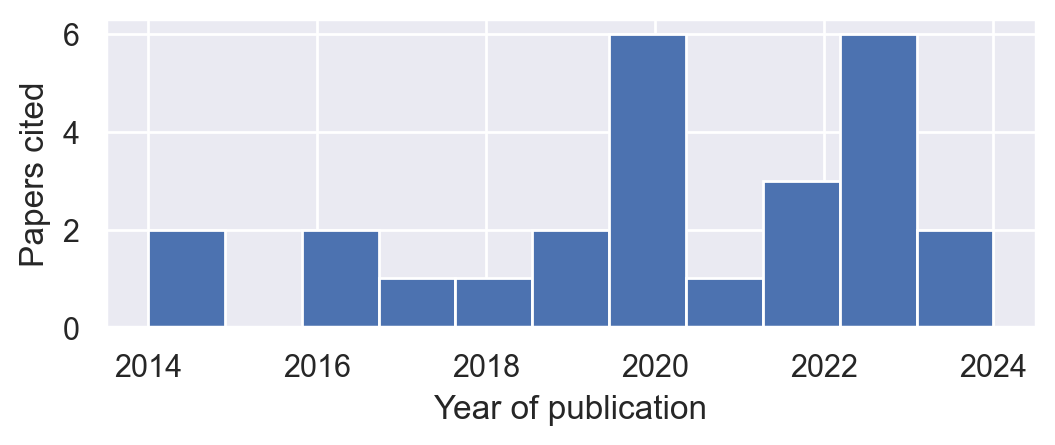
\includegraphics[height=90pt]{years_reference.png}
	\caption{Year of publication of papers cited in this thesis. These topics are novel!}
\end{figure}

One of the main strengths of my work in this thesis was having built a solid experimentation infrastructure early on, which allowed me to iterate quickly on experiments and ideas.
The program to build, run, and analyse the counterparametric-enhanced queries (which is present in \cref{appendixD} and in this project's repository) is one of the strong points of this project, and I'm sure it will be a valuable tool in future research projects.

Despite settling on the final thesis idea early, this thesis suffered from lacking a clear and well-defined research question, which emerged late in the process.
I consider this delay to have been one of the main sources of inefficiencies, since it lead to executing long experiments that contributed little to the final thesis.
One of my main takeaways from this research is the necessity to align on a well-defined research question early.

This thesis taught me how to adapt to the rapidly-changing research landscape of sequence analysis and artificial intelligence.
A lot of the methods used in this work are taken directly from previous academic papers, and this allowed me to test my hypothesis quickly while keeping a deep understanding of the context I am working on.

Most of all, I'm happy to have learned a lot about the areas of large language models and  to have been able to collaborate a bit in this very new area of research.
I plan to continue this work in the future, and I'm looking forward to contributing to the research on this area!

\subsection{Future Work}

\subsubsection{Better Categorisation of the Answers}
\label{other_problems}

To test whether two answers are equal and to know whether an answer came from parametric or contextual knowledge, the code in this thesis checks for string equality among after removing a few stop simple words such as `the'.

This solution might not be enough, and some answers classified as \Other{} should have been classifier as something else.
\Cref{bad_others} provides some examples of answers where the answer should have been categorised as \Parametric{} or \Contextual{}.

\begin{table}[ht]
	\centering
	\scriptsize
	\begin{tabular}{>{\ttfamily}l@{\hspace{20pt}}>{\ttfamily}c@{\hspace{1pt}}>{\ttfamily}c@{\hspace{1pt}}c@{\hspace{1pt}}c}
		\toprule
			\bfseries \rmfamily Query & \bfseries \rmfamily Parametric Answer & \bfseries \rmfamily Query Answer & \bfseries Comparison & \bfseries Expected \\
		\midrule
			\parbox[c][100pt][t]{120pt}{[Context: The primary leader associated with The Construction of Hadrian's Wall was Napoleon Bonaparte] \\ Q: Who was the primary leader associated with The Construction of Hadrian's Wall? \\ A: The primary leader associated with The Construction of Hadrian's Wall was} &
			Emperor Hadrian &
			\parbox{75pt}{\centering Hadrian, \\ the Roman Emperor} &
			\bfseries \textcolor{MidnightBlue}{Other} &
			\bfseries \textcolor{ForestGreen}{Parametric} \\
			\parbox[c][85pt][b]{120pt}{[Context: Che Guevara was born in Kensington, London, England] \\ Q: In what city was Che Guevara born? \\ A: Che Guevara was born in \\} &
			Rosario, Argentina &
			London &
			\bfseries \textcolor{MidnightBlue}{Other} &
			\bfseries \textcolor{Maroon}{Contextual} \\
		\bottomrule
	\end{tabular}
	\caption{Example of incorrectly-categorised answers. These were categorised as "\Other{}", since their answer strings are different from both parametric and contextual answers. However, a closer look reveals that this is just a \Parametric{} or \Contextual{} answer with a slight formatting difference.}
	\label{bad_others}
\end{table}

A more complete solution might include using another LLM to compare whether two answers are truly equal.

\subsubsection{Knowledge Grounding in Retrieval-Augmented LMs}

This thesis was originally based on a preprint, ``Knowledge Grounding in Retrieval-Augmented LMs: An Empirical Study'' \citep{knowledge_grounding_retrieval_augmented}, and contains work towards understanding how large language models retrieve data which can ultimately help prevent hallucinations.

We plan to continue this work and complete the paper created by the preprint by running the methods outlined on this thesis on retrieval-augmented LMs such as \textsc{Atlas} \citep{atlas_foundational} and \textsc{Retro} \citep{retro} and creating a full evaluation framework that specifically focuses on their grounding.
A well-grounded model should demonstrate the capability to adapt its generation based on the provided context, specially in cases like the ones experimented in this thesis when the context contradicts the model's parametric memorisation, and we can experiment with an analysis similar to the one done in this thesis for those models.

\subsubsection{Fine-tuning a LLM for a RAG Context}

In this research we proved that certain models architectures are preferable to others for answering from data from the context when it contradicts the parametric knowledge of a model.

Existing retrieval-augmented language models, such as \textsc{Atlas} and \textsc{Retro}, are trained on existing models along with an index.
We can continue this approach by fine-tuning an existing LLM, such as the \texttt{Flan-T5} or Llama models used in this thesis, specifically to be able to answer these kinds of queries better.
